

% change this to false to remove the appendix
%\setboolean{with_appendix}{false}

Word embedding models are increasingly being used in communication research to measure categories of interest in media content analyses \parencite[e.g.,][]{Rudkowsky2018}. They allow  various applications ranging from simple synonym detection to detecting shifts in the meaning of specific words over time \parencite{wiedemann2021}. One such application is the assessment of implicit stereotypical associations \parencite[ISAs;][]{greenwald1998measuring} within large text corpora \parencite{durrheim2023}. Earlier research on word embedding models trained on large, human-generated data sets found them to mirror cultural stereotypes or biases held by society at large. For example, it has been shown that models trained on large text corpora tend to associate occupation words like \textit{nurse} with women and \textit{engineer} with men {\parencite{bolukbasi2016}}. So called ``word embedding association'' metrics have been proposed to quantify the degree to which ISAs occur in a word embedding model \parencite{caliskan:2017:S}. 

While word embedding-based methods such as word embedding association tests (WEATs) were originally conceptualized for the application of finding unwanted associations within a word embedding model \parencite[also sometimes referred to as ``biases'' within the models, see e.g.,][]{caliskan:2017:S}, word embedding-based metrics are now increasingly being used as a content analysis tool \parencite{kroon2021,sales2019media,andrich:2023:GGS,andrich2022leader,fu:2023:PRG,mueller:2023:DRN,urman:2022:F,azzalini:2025:CI}: Instead of detecting unintended associations that a word embedding model might have inherited from its training corpus, the goal in this field of application is to train a word embedding model on an analysis corpus of interest to investigate ISAs that occur within this corpus to draw conclusions about the corpus' semantic content \parencite{durrheim2023}. This application is based on the (often unstated) assumption that ISAs measured based on word embedding models correspond to the actual implicit stereotypes conveyed to human readers by the texts contained in the corpus.

But, when researchers apply word embedding models for the task of measuring ISAs within corpora, they may ask themselves whether this assumption is actually correct---that is: would human readers detect the same associations in a text corpus that word embedding-based statistics suggest? Considering the increasing number of applied content analytical studies using word embedding-based measures of ISAs in mediated messages, establishing these measures' validity is a crucial task. However, while there is already some prior evidence on their predictive and face validity \parencite[for a summary, see,][]{durrheim2023}, it is still an open question whether word embedding-based ISA measures are actually semantically valid. That is, it is unclear whether the ISAs measured with these scores conform to implicit stereotypes that the assessed corpus conveys to a human readership. Without testing for semantic validity, word embedding-based ISA measures run the risk of creating methodological artifacts that might be internally consistent and correlate with external data, but might still represent texts in a way that is not in line with human understanding of these same texts.

Therefore, in this article, we develop and conduct a routine for testing the semantic validity of word embedding-based ISA measures. This is not a straightforward task. In media content analysis, researchers typically use measures that are located at the text or sentence levels. This allows them to conduct semantic validation by comparing ``gold-standard'' manual coding data generated by human coders to automated measures of the same categories \parencite{Grimmer2013,song:2020:ivw}. However, this way of testing for semantic validity is not feasible with word embedding-based scores as they are based on a whole, typically rather large, text corpus. It is unrealistic to let human coders read hundreds of thousands of sentences and hope for a summarizing judgment on them in their totality. We suggest an alternative approach by developing and applying an experimental survey approach that is tailored to the semantic validation of word embedding-based ISA measures. 

In the following, we will first describe how word embedding-based metrics have recently been used in communication research to assess implicit stereotypical associations conveyed within texts. We, then, review the current state of knowledge about the validity of this application, and make a case for the importance of establishing its semantic validity (which is yet lacking). Subsequently, we discuss the difficulties of assessing semantic validity  a corpus- based content analytical measure and present our experimental survey approach for moving on with this task. We demonstrate the usefulness of our approach by validating a specific case in which ISA measures based on static word embeddings have been used to assess group stigmatization in news messages \parencite{mueller:2023:DRN}. This validation study (1.) offers first insights into the semantic validity of using word embedding-based metrics to assess ISAs in large text corpora and (2.) can serve as a blueprint for future attempts to validate word embedding-based measures in other use cases within the realms of media content analysis. Importantly, its substantial findings are limited to the validated application. Additional semantic validation studies, also considering newer contextual word-embedding approaches, will necessarily have to follow.

\section{Word Embedding-Based ISA Measures and Their Validity}

\subsection{Word Embedding-Based ISA Metrics}

Word embeddings are trained on a large corpus of texts in an unsupervised manner, usually as a by-product of training a neural network to predict a word using other words surrounding it. This by-product can be used to quantify the semantic meanings of words based on the linguistic properties of distributional semantics. Word embeddings work by utilizing co-occurrence statistics to place all unique words in a corpus on multidimensional word embedding spaces. Each row in these spaces represents the word vector of one word. For example, words like \textit{fluid} and \textit{water} are more likely to occur in the same sentence as \textit{flow}, while words like \textit{solid} or \textit{steel} are less likely to do so \parencite{pennington:2014:G}. For words with a similar semantic meaning (e.g., \textit{fluid} and \textit{water} in the above example) their similarity can be quantified by comparing their word vectors. By the same token, words with different meanings (e.g., \textit{water} and \textit{steel}) should have very different word vectors. Therefore, the comparability of word vectors is able to tell us which words are more closely associated. In communication research, this comparability was originally used to enhance supervised and unsupervised machine learning models over the traditional ``bag-of-words'' model \parencite[e.g.,][]{Rudkowsky2018,atteveldt:2021:VSA}. There exist several pretrained word vectors that researchers can use in an off-the-shelf manner.

However, this application has also been criticized because pretrained word embeddings might contain unwanted associations inherited from the texts in their training corpora, so that a downstream task would also be tainted by those associations. Pioneer works in this regard are \textcite{caliskan:2017:S} and \textcite{garg:2018:W}. These studies derived several ``word embedding association'' metrics to quantify what the authors interpret as ``biases'' in pretrained word vectors. These metrics are also based on the comparability of word vectors: the relative similarity in the word embedding space of a target (e.g., \textit{nurse}) with different attributes (e.g., \textit{male} and \textit{female}) can tell us how the word vectors---and by extension, their original training corpus---represent different target entities to be implicitly associated with other entities. 

More recently, this approach has been extended as a computational communication research method to assess implicit stereotypical associations within text: Instead of using pretrained word vectors, word embeddings are trained on a large corpus of texts that one wants to study. Resulting word embedding association metrics are used to quantify ISAs in the corpora---which have in past research been interpreted as ``stereotypes''~\parencite{kroon2021,andrich:2023:GGS,andrich2022leader,azzalini:2025:CI}, ``media bias''~\parencite{sales2019media,curto:2022:AA}, or ``implicit representations/ associations''~\parencite{fu:2023:PRG,mueller:2023:DRN,urman:2022:F}. In this kind of application, word embedding-based metrics are not used to assess potential biases within a word embedding model with the aim to reduce these biases. Instead, they are used as a content analysis tool: Researchers calculate word embedding-based scores to make observations about the corpora they train the model on. However, while the body of applied studies employing word embedding-based ISA metrics is flourishing \parencite[also see,][]{durrheim2023}, these applications yet lack a demonstration of their semantic validity.

\subsection{The Missing Semantic Validity of Using Word Embedding-Based ISA Metrics for Content Analysis}
\textcite{dimaggio:2013:E}, \textcite{quinn:2010:HAP}, and \textcite{Grimmer2013} conceptualize three different aspects of validation in automated text analysis: statistical, predictive, and semantic. These three aspects supplement each other. Statistical validity indicates whether results generated from a model agree with the model's statistical assumptions. Usingword embedding-based ISA metrics as an example, the stability of the measurement is one aspect of this statistical assumption. It can be assessed using standardized tests \parencite[e.g.,][]{spliethover2021bias}. Statistical validity \textit{per se} is important but not sufficient as sole evidence of the validity of a measure because it evaluates only the internal coherence of a model. 

Predictive validity, on the other hand, measures the ``expected correspondence between a measure and exogenous events uninvolved in the measurement process'' \parencite[][p. 222]{quinn:2010:HAP}. Foundational works on word embedding-based ISA measures established the validity of the approach primarily in terms of predictive validity \parencite[for an overview see,][]{durrheim2023}. For instance, \textcite{caliskan:2017:S} show the correlation between WEAT-based scores derived from word vectors trained on Wikipedia and various web corpora \parencite{pennington:2014:G} with Implicit Association Test (IAT) scores obtained from some exogenous U.S. experiments conducted in the 1990s \parencite{greenwald1998measuring}. Similarly, \textcite{garg:2018:W} validate word embedding-based scores on gender biases in occupation within a Google News corpus by testing their correlation with the relative percentage of females in different occupations in the U.S. in the 1960s. For use cases in which word embedding-based ISA metrics are employed to detect biases within word embedding models and de-bias them for further application, this correspondence of these metrics to external data suffices.

In recent years, though, word embedding-based measures have been used to assess stereotypical associations within texts from specific periods and regions. For example, \textcite{kroon2021} aim to show that ``representations of minorities in newspapers have become progressively remote from factual integration outcomes, and are therefore rather an artifact of news production processes than a true reflection of what is actually happening in society.'' Their claim is that the associations measured within a word embedding model trained on news do not correspond to external data, but instead indicate a stereotypical portrayal within the news corpus. Word embedding-based scores are here used as a content analysis tool: The researchers' goal in this kind of application is to make assertions about the content of news in the observed corpus, not about external society. To validate the application of word embedding-based scores for these kinds of applications, predictive validity does not suffice---in fact, where one expects a divergence between reporting and external societal phenomena, predictive validity cannot be used to assess the method's validity at all.

Therefore, when using word embedding-based metrics as a content analysis tool, one needs to supplement statistical and predictive validity with semantic validity. \textcite[][p.323]{krippendorff2018content} defined semantic validity as ``the degree to which the analytical categories of texts correspond to the meanings these texts have for particular readers or the roles they play within a chosen context.'' An important distinction between predictive validity and semantic validity is therefore what the measure of interest corresponds to: The ground truth in the case of semantic validity is the human understanding of texts, rather than some exogenous cultural patterns. One can therefore consider semantic validity a form of criterion validity, where the criterion test---more commonly referred to as ``gold standard'' \parencite{song:2020:ivw,atteveldt:2021:VSA,lind:2017:CAC}---is the human understanding. Consequently, semantic validity as a category is much closer to the actual target construct that is supposed to be measured in text analysis, namely the meaning conveyed by text to human readers, than predictive validity. 

Krippendorff's works refer to manual content analysis with human coders. In this context, they suggest to compare human coders' ratings of media content to that of individuals with expertise in the field under study \parencite[political professionals for political texts, legal experts for legal texts etc.][]{krippendorff1980}. In the present study, instead of focusing on topical experts to produce the criterion values for semantic validity, we use a slightly different approach and examine a general media audience's assessment. In manual content analysis, trained coders are typically not such experts, but rather resemble members of the general media audience. Therefore, the question whether their coding is in line with the general audience's understanding of texts appears less pressing. For automated analysis, the case is different. Here, it is far from self-evident that the analysis routines produce a textual understanding that coincides with that of the general media audience.

However, this question is important when we consider the epistemological focus that content analytical assessments are typically conducted with. There are two inferential goals of media content analysis: (1.) the ``diagnostic approach'' is interested in making inferences about media messages' production circumstances from content analysis, (2.) while the ``prognostic approach'' tries to infer predictions of a message's potential processing and effects \parencite[][p. 13]{maurer2006}. The latter is especially important in the context of ISAs because of the harm that these kinds of messages might do to societal intergroup relations. Therefore, when establishing word embedding-based ISA assessment's semantic validity we are particularly interested in whether its substantial findings are in line with a general audiences' impression of the same content. This is a logical prerequisite to inferring predictions of media processing and effects from the content analytical results obtained by these measurements.

\subsection{The Challenges of Semantic Validation---And How to Address Them}

For common automated content analysis techniques such as sentiment detection or topic modeling, the units of analysis are typically articles or their sub-units such as sentences or paragraphs. Therefore, it is relatively easy to compare measures extracted for these units, for instance their  sentiment scores or topic allocations, with assessments of the same categories made by human coders. It is also possible to test the semantic validity of the measure by studying a representative sample of articles in the corpus. Although the amount of sampled articles does impact the validation outcome \parencite{song:2020:ivw}, it is indeed statistically valid \parencite{krippendorff2018content} and the approach has been recommended in the methods literature \parencite{Grimmer2013,,atteveldt:2021:VSA,lind:2017:CAC} and widely used in computational communication research.

However, word embedding-based ISA measures represent the word associations in an entire corpus and are therefore aggregated text measurements at the corpus level. The resulting scores cannot be broken down into single texts, paragraphs, or even sentences as units of analysis. Consequently, semantic validation that would compare word embedding-based scores with human-generated data of the same texts has previously not been applied when attempting to validate the method's suitability for assessing ISAs within text. \textcite[][p. 409]{mueller:2023:DRN} even explicitly pointed out that a validation using human coding is impractical. In their analysis of implicit stereotypical associations of ethnic and religious group names with emotions, the authors assert that ``[a] proper human validation would need raters to read the entire corpus of 697,913 articles and point out what racial biases they have learned from the corpus.'' For a similar method, \textcite[][p.13]{arendt2017content} defend the decision not to validate their measurement because ``there is no real `gold standard' of what the `true' mediated associations are.'' These assertions underscore the difficulty, but do not rule out the possibility for validating word embedding-based ISA measures. However, such an attempt cannot follow the same logic and approach as the semantic validation of text- or sentence-based measurements. For an entire corpus, it is impractical to use the so-called ``gold standard'' procedure of asking trained human coders to go over the texts under study and ask them to manually code ISAs as observational evidence of word embedding-based scores' semantic validity.

A practical approach to overcome these issues, according to \textcite[][p.409]{mueller:2023:DRN}, is ``to develop ways of validating word embedding bias methods using a well-defined causal conjecture.'' Applying this logic, one can first propose a causal conjecture in the form of hypotheses and then test them empirically. A suitable causal conjecture for semantically validating word embedding-based ISA measures is that a sentence package with stronger ISAs for a specified entity (as measured by word embedding-based scores) \textbf{causes} human readers to perceive that the sentence package contains such associations to a higher extent than a control condition. This causal conjecture can be studied using an experimental research design \parencite{imai2011}. In fact, a similar approach (using experimental designs to establish semantic validity) was proposed and applied in the early days of computational text analysis to study the validity of topic models by \textcite{Grimmer2013,grimmer:2011:G}.

In transferring the notion of semantic validation via survey experiments to the case of word embedding-based scores, we propose a routine which proceeds in three steps: 
\begin{enumerate}
    \item As we cannot expect human participants to read a complete corpus, we extract different packages of sentences from a previous study's corpus \parencite{mueller:2023:DRN} that we expect to contain ISAs.
    \item Then, we ensure that word embedding-based scores capture the ISAs assumed to be present in those sentences. We inject the sentence packages into a version of the original corpus that is stripped of all other mentions of the target group to remove the original ISA from the corpus. This modified corpus is used for assessing the level of ISAs in sentence packages.
    \item  Finally, we conduct an experimental study in which we let a large sample of human participants read scaled-down versions of the different sentence packages and afterwards ask them to answer a set of survey questions tailored to capture the ISAs conveyed by these sentences. If the results on these survey measures are in line with word embedding-based measures of ISAs, the causal conjecture established by the experimental design offers an argument for the semantic validity of using word embeddings to investigate ISAs in large text corpora.
\end{enumerate}

By conducting this validation procedure in an experimental survey setting instead of hiring a limited number of trained coders (as in the typical gold standard validation routine), we make use of the law of large numbers. In contrast to the traditional coding approach in which each unit of analysis is judged by one coder \parencite[also the one applied in crowd coding, see, e.g.,][]{atteveldt:2021:VSA,lind:2017:CAC}, the same sentence packages are evaluated by large groups of individuals. Instead of one data point per text unit, we, thus, gather a large number of data points on the same units. This accounts for the fact that implicit meanings such as ISAs may be perceived differently by various human readers, even by trained coders. Considering this variance, we assess the average meaning conveyed by different sentence packages to humans based on a large amount of data points. Further, contrary to a typical coding scheme the survey approach can account for the implicit nature of conveyed ISAs by using various text-dependent measures as indicators, not just one (single-item) assessment that is typically used to capture (quasi-)manifest textual meanings by human coders.

\section{Study Design}

We preregistered the hypotheses, survey, and analytical plan for this study before data collection. The code to reproduce both the stimulus generation process and the obtained survey data can be found on OSF.\footnote{All materials can be found at: \url{https://doi.org/10.17605/OSF.IO/TQRJ3}} All Appendices are available in the same repository. 

\subsection{Case}

We designed this study based on the Open Science materials shared by \textcite{mueller:2023:DRN}. In that study, word embedding-based ISA metrics were applied to assess implicit stigmatization of ethnic and religious groups in German news reporting by measuring the co-occurrence of group labels with words implicitly charged with the positive emotion admiration or the negative emotion fear. Importantly, in the original study, this measurement was conducted based on a non-``pretrained'' word embedding model. Instead, it was trained from the study's own text corpus using the GLoVE algorithm.

For the present validation attempt, our goal was to create three artificial stimulus sentence packages---one consisting of sentences that implicitly associate a target group with fear, one implicitly associating the same group with admiration, and one that contains no implicit association of the target group with either of the two emotions (control condition). For the generation of sentence packages, we used a group (Italian people) that Müller et al. (\citeyear{mueller:2023:DRN}) found to be portrayed in a balanced way on average within the corpus. We reasoned that an overall balanced group portrayal meant we would find enough sentences that implicitly contained either admiration or fear. Additionally, if we assume that the found associations within the original study are somewhat representative of stereotypes the wider population has internalized, it should be easier to construct an intuitively credible implicitly biased dataset based on this group. For example, using a group that is stereotypically associated with fear and constructing an artificial corpus where this group is implicitly associated with admiration might result in a failure of the validation attempt because existing stereotypes are less malleable and the sentences are therefore perceived as unrealistic or implausible by participants.

Following \textcite{mueller:2023:DRN,urman:2022:F}, we used the normalized association score ($NAS$) \parencite{caliskan:2017:S} to quantify ISAs. $NAS$ is calculated with the word embeddings $\boldsymbol{w}$, target words $\boldsymbol{s}$, admiration attribute wordset $\mathcal{A}$, and fear attribute wordset $\mathcal{B}$ (See Appendix A in the OSF repository). The software implementation by \textcite{chan:2022} was used.

%% notion: attributes wordset \mathcal{A} \mathcal{B} are mathematical sets, in R it was represented as vectors. Capitalized stuff has more than one values; target $s$ is a single word; targets (multiple words, as we used in the PolComm paper) can be represented as target wordset \mathcal{S}.
%% \mathcal is a set; \mathbf is a vector

Suppose the cosine similarity score between word $a$ and $b$ in the word embedding space of $\boldsymbol{w}$ is denoted as $cos(\boldsymbol{w_a}, \boldsymbol{w_b})$.

\begin{equation}
cos(\boldsymbol{w_a}, \boldsymbol{w_b}) = \frac{\boldsymbol{w_a} \cdot \boldsymbol{w_b}}{ || \boldsymbol{w_a} || || \boldsymbol{w_b} ||}
\end{equation}

For a given word $s$, let us denote its differential association with $\mathcal{A}$ and $\mathcal{B}$ as $g(s, \mathcal{A}, \mathcal{B}, \boldsymbol{w})$. And it is calculated as:

\begin{equation}
g(s, \mathcal{A}, \mathcal{B}, \boldsymbol{w}) = \frac{1}{|\mathcal{A}|} \sum\nolimits_{a \in \mathcal{A}} cos(\boldsymbol{w_s}, \boldsymbol{w_a}) - \frac{1}{|\mathcal{B}|} \sum\nolimits_{b \in \mathcal{B}} cos(\boldsymbol{w_s}, \boldsymbol{w_b})
\end{equation}

The mean of all cosine similarity scores of the union of $\mathcal{A}$ and $\mathcal{B}$ of a given word $s$ is denoted as $m(s, \mathcal{A}, \mathcal{B}, \boldsymbol{w})$. It is calculated as:

\begin{equation}
m(s, \mathcal{A}, \mathcal{B}, \boldsymbol{w}) = \frac{1}{|\mathcal{A} \cup \mathcal{B}|} \sum\nolimits_{x \in \mathcal{A} \cup \mathcal{B}} cos(\boldsymbol{w_s}, \boldsymbol{w_x})
\end{equation}

And the standard deviation $\sigma(s, \mathcal{A}, \mathcal{B}, \boldsymbol{w})$ is calculated as:

\begin{equation}
\sigma(s, \mathcal{A}, \mathcal{B}, \boldsymbol{w}) = \sqrt{\frac{1}{|\mathcal{A} \cup \mathcal{B}| - 1} \sum\nolimits_{x \in \mathcal{A} \cup \mathcal{B}} (cos(\boldsymbol{w_s}, \boldsymbol{w_x}) - m(c, \mathcal{A}, \mathcal{B}, \boldsymbol{w}))^2}
\end{equation}

The $NAS$ of word $s$ is denoted as $NAS(s, \mathcal{A}, \mathcal{B}, \boldsymbol{w})$:

\begin{equation}
NAS(s, \mathcal{A}, \mathcal{B}, \boldsymbol{w}) = \frac{g(s, \mathcal{A}, \mathcal{B}, \boldsymbol{w})}{\sigma(s, \mathcal{A}, \mathcal{B}, \boldsymbol{w})}
\end{equation}

In \textcite{mueller:2023:DRN} and in the original implementation by \textcite{caliskan:2017:S}, the target is also a wordset $\mathcal{S}$, e.g., all grammatical forms of an ethnic group label $\{ Italiener,  Italienerin, \ldots \}$. $NAS(\mathcal{S}, \mathcal{A},\mathcal{B}, \boldsymbol{w})$ is the average of all $NAS(s_{i}, \mathcal{A}, \mathcal{B}, \boldsymbol{w})$ of all targets words $s_{i}$ in $\mathcal{S}$. For the current experimental setting, we used one target word (\textit{Italiener}, the singular or plural male nominative form) only. Therefore, $NAS(\mathcal{S}, \mathcal{A}, \mathcal{B}, \boldsymbol{w})$ and $NAS(s, \mathcal{A}, \mathcal{B}, \boldsymbol{w})$ are identical.

\subsection{Preregistered Hypotheses}

Our goal was to test whether the ISAs picked up by word embedding-based scores are conveyed to a human audience. Accounting for the implicit nature of the associations to be assessed, we attempted to establish this semantic validity based on a larger set of measures that may all be causally linked to implicit associations of the target group with admiration or fear in the stimulus sentence packages. We supposed that the more of the following preregistered hypotheses\footnote{Parts of the hypotheses were re-phrased during manuscript preparation to better specify the intent of the study. This, however did not affect the relationships under study, labeling of outcome variables or directions of assumed effects. The original ideas of the hypotheses are still fully represented. For full disclosure, the original versions of the pre-registered hypotheses are available via the OSF repository associated with this study. The preregistration included a seventh hypothesis about assumed message effects as a dependent variable ("Assumed message effects will be stronger for corpora containing ISAs with fear or admiration as indicated by WEAT-based measures, compared to a corpus with no ISA"). Analysis of this hypothesis was omitted from the present manuscript for the sake of brevity. However, respective results can be obtained from the Online Appendices published in this study's OSF repository.} were supported, the stronger the evidence for the semantic validity of word embedding-based ISA measures was:

\begin{description}
\item[H1:] \emph{If word embedding-based measures indicate that a sentence package contains an ISA of a target group with fear, the representation of this target group will be perceived as more negative (compared to a corpus with no ISA).}

\item[H2:] \emph{If word embedding-based measures indicate that a sentence package contains an ISA of a target group with fear, the representation of this target group will be perceived as more negative (compared to a corpus with an ISA with admiration).}

\item[H3:] \emph{If word embedding-based measures indicate that a sentence package contains an ISA of a target group with admiration, the representation of this target group will be perceived as more positive (compared to a corpus with no ISA).}

\item[H4:] \emph{If word embedding-based measures indicate that a sentence package contains an ISA of a target group with admiration, this target group will be perceived as (a) more admirable and as (b) less frightening (compared to a corpus with no ISA).}

\item[H5:] \emph{If word embedding-based measures indicate that a corpus contains an ISA of a target group with admiration, this target group will be perceived as (a) more admirable and as (b) less frightening (compared to a corpus with an ISA with fear).}

\item[H6:] \emph{If word embedding-based measures indicate that a sentence package contains an ISA of a target group with fear, this target group will be perceived as (a) more frightening and as (b) less admirable (compared to a corpus with no ISA).}

\end{description}

\subsection{Semantic Validation Procedure}

As outlined above, establishing semantic validity of an automated content analytical measure means to assess whether its results are mirrored in human readers' judgments of the same texts. In the case of word embedding-based metrics which can only be calculated for large text corpora, it is nearly impossible to have human study participants read the full textual material that these measures are rating. We also usually do not know the sentences that introduce a specific association in the models. It is therefore not straightforward to arrive at a diminished corpus which could be processed by human readers. But by the means of reverse engineering, we can attempt to reproduce those sentences within a corpus that probably contributed to the measured association expressed in scores derived from a word-embedding model which was trained on said corpus. We can, then extract those sentences from the corpus, and use them to be rated by human study participants. 

As previously outlined, our semantic validation routine followed this three-step process which we will describe in more detail in the following. The overall procedure for generating the sentence packages and testing their WEAT-based association scores within a large corpus is visualized in Figure \ref{fig:flowchart}. In addition to that, the table displayed in Appendix B offers a concise overview of the consecutive steps of text processing. We explain these individual steps in more detail in the following subsections.

\begin{knitrout}
\definecolor{shadecolor}{rgb}{0.969, 0.969, 0.969}\color{fgcolor}\begin{figure}
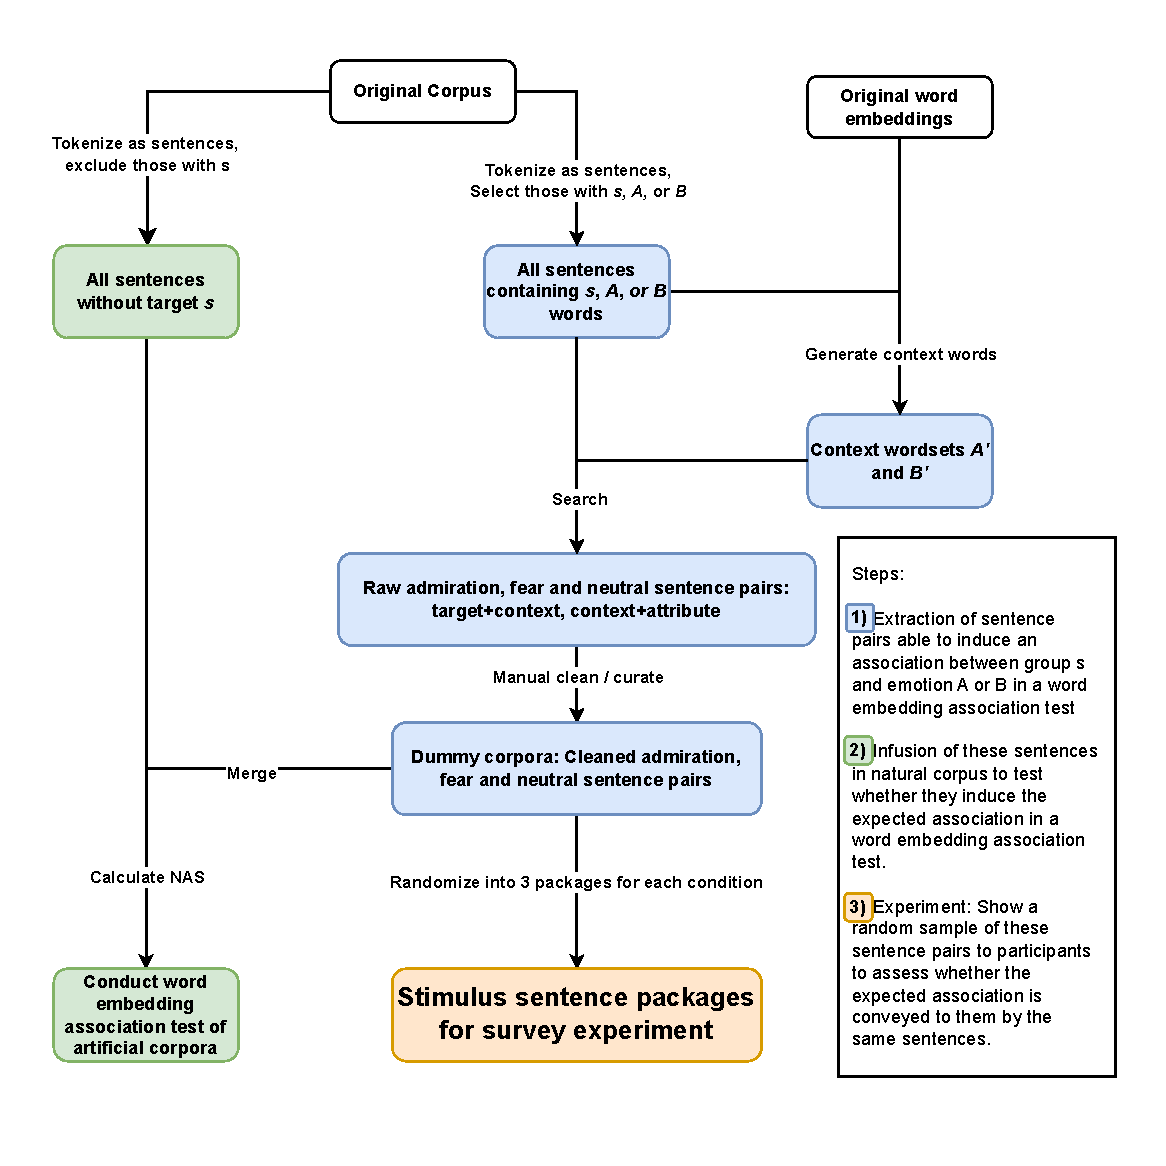
\includegraphics[width=\maxwidth]{intermediate/wevarticle.drawio} \caption[Flowchart of the stimulus sentence package generation process]{Flowchart of the stimulus sentence package generation process}\label{fig:flowchart}
\end{figure}

\end{knitrout}

\subsubsection{Step 1: Identifying Potentially ISA-Inducing Sentence Packages}

The idea behind implicit associations within word embeddings is that certain wordsets represent specific concepts. In the present study's context, wordset $\mathcal{A}$ represents fear and wordset $\mathcal{B}$ represents admiration. They comprise of words that explicitly contain said concepts, such as \textit{scary} or \textit{admirable}. Then, there are sets of context words ($\mathcal{A'}$ and $\mathcal{B'}$, such as \textit{crime} or \textit{actor}). These context words often co-occur with the words included in the explicit wordset of the respective concept (e.g., \textit{actor} often co-occurs with words such as \textit{admirable}). An implicit association with $\mathcal{A}$ or $\mathcal{B}$ occurs, then, when a target group $s$ is often mentioned close to those context words. For instance, if \textit{Italian} often co-occurs with context words such as \textit{actor} but less so with explicit concept words such as \textit{admirable}, the group of \textit{Italians} would be indirectly---or: implicitly---associated with the concept admiration. If present, such ISAs can be measured using $NAS$ scores calculated from a word embedding model that was trained on a corpus of interest. This is how $NAS$ can be used to operationalize ISAs in text corpora.

To validate this operationalization, in a first step, we generated packages of sentences that established such an implicit association between a group name and the two emotions fear and admiration from the original study's corpus \parencite{mueller:2023:DRN}. For this purpose, two sentences are required: One that links a context word with an explicit emotion word (thereby, charging the context word with the respective emotion) and one that links a target group with a context word (thereby, implicitly charging the group label with the respective emotion). Such a sentence pair, for instance, looks like this: 

\begin{itemize}
    \item \textit{The Italian actor keeps personal matters private and rarely discusses family life.}
    \item \textit{Audiences were moved by the actor’s admirable portrayal of a young musician.}
\end{itemize}

These two sentences establish an implicit association between the target $s$ (\textit{Italian}) and the attribute admiration (\textit{admirable}), because a context word (\textit{actor}) co-occurs with both. The first sentence is an example of a target-context association sentence, in which the target is associated with a context. The second sentence is an example of a context-attribute association sentence, in which the context is associated with an attribute. 

An example for the implicit association with fear is:

\begin{itemize}
    \item \textit{The Italian from the Left Party blamed the government for the escalation.}
    \item \textit{The mayor fears an escalation of violence in the region.}
\end{itemize}

In this example, the context word \textit{escalation} co-occurs with an explicit \textit{fear} word as well as with the group label \textit{Italian}. Importantly, to establish an implicit rather than an explicit link between the concepts, these linking sentences do not occur close to each other or even within the same documents of a text corpus, but are distributed across several texts within the corpus. 

In stimulus sentence package construction, the overarching goal therefore was to look for context words (e.g., $\mathcal{A'}$) that co-occur with attribute words (e.g., $\mathcal{A}$), in context-attribution association sentences, and that co-occur with the target ($s$) in target-context association sentences which are otherwise free from evaluative language. Using the word embedding model and the wordsets for $\mathcal{A}$ and $\mathcal{B}$ provided in \textcite{mueller:2023:DRN}, we generated a list of context words that are not contained in $\mathcal{A}$ or $\mathcal{B}$, but co-occur with both.

To identify context words, we selected terms that are (1) semantically close to the words in $\mathcal{A}$ and $\mathcal{B}$, but not those words themselves, and (2) also semantically distant from the opposite wordset: $\mathcal{A'}$ are terms close to $\mathcal{A}$, but distant from $\mathcal{B}$; $\mathcal{B'}$ are terms close to $\mathcal{B}$, but distant from $\mathcal{A}$. We applied the SemAxis technique by \textcite{an2018semaxis} to find these context words. First, we calculated the column mean vectors $\mathbf{V}^{\mathcal{A}}$ and $\mathbf{V}^{\mathcal{B}}$ of all word vectors of words in $\mathcal{A}$ and $\mathcal{B}$ respectively as:

\begin{equation}
\mathbf{V}^{\mathcal{A}} = \frac{1}{|\mathcal{A}|} \sum\nolimits_{a \in \mathcal{A}} \boldsymbol{w_a}
\end{equation}

\begin{equation}
\mathbf{V}^{\mathcal{B}} = \frac{1}{|\mathcal{B}|} \sum\nolimits_{b \in \mathcal{B}} \boldsymbol{w_b}
\end{equation}

Subtracting $\mathbf{V}^{\mathcal{B}}$ from $\mathbf{V}^{\mathcal{A}}$ gives the semantic axis vector $\mathbf{V_{axis}}$. 


\begin{equation}
\mathbf{V_{axis}} = \mathbf{V}^{\mathcal{A}} - \mathbf{V}^{\mathcal{B}}
\end{equation}

Given a word $c$ and its word vector $\boldsymbol{w_c}$, we calculated $cos(\boldsymbol{w_c}, \mathbf{V_{axis}})$ for all words covered in $\boldsymbol{w}$. We selected a word $d$ in $\mathcal{A'}$ if it satisfied the following criteria: (1) $d$ co-occurs with $s$ in a sentence of the corpus; (2) $d$ is not in $\mathcal{A}$; and (3) $\boldsymbol{w_d}$ has a high cosine similarity to $\mathbf{V_{axis}}$. For $\mathcal{B'}$, the criteria are the same, except we selected a word $d$ which has a low cosine similarity to $\mathbf{V_{axis}}$\footnote{Another way to think about this is to calculate the semantic axis vector as $\mathbf{V_{-axis}} = \mathbf{V}^{\mathcal{B}} - \mathbf{V}^{\mathcal{A}}$ and look for word $d$ with a high $cos(\boldsymbol{w_d}, \mathbf{V_{-axis}})$.} and not in $\mathcal{B}$. For $\mathcal{A'}$ and $\mathcal{B'}$, we selected the top 200 words according to their cosine similarity scores.

Using $s$, $\mathcal{A}$, $\mathcal{B}$ provided by \textcite{mueller:2023:DRN} and the created context wordsets $\mathcal{A'}$ and $\mathcal{B'}$, we searched the original corpus for matching pairs of target-context association and context-attribute association sentences for the admiration and fear conditions. In addition to these two sentence packages, we also deemed it useful for the purpose of our survey experiment to have a sentence package in which no implicit or explicit association between the target group and the two emotions fear and admiration was established. This neutral sentence package should then serve as a control condition in the experimental setting. As control sentences, we selected pairs in which one sentence contained only $s$ and no words from $\mathcal{A}$, $\mathcal{B}$, $\mathcal{A'}$ nor $\mathcal{B'}$ plus one sentence containing neither $s$, nor words from $\mathcal{A}$, $\mathcal{B}$, $\mathcal{A'}$ nor $\mathcal{B'}$).
 
We found that this method did not generate an amount of sentence pairs that associated the selected group label `Italian' with the concept fear that was sufficient for the purposes of our study. Therefore, we drew sentences for a similar group label (\textit{Spanish}), and replaced this group name with \textit{Italian} in all sentences. Thus, we created 347 sentence pairs for each condition. To make the final data set semantically meaningful for human readers, we manually removed duplicates, rephrased fragmentary and incoherent sentences, and arrived at one sentence-pair dummy corpus for each condition.

\subsubsection{Step 2: Measuring ISAs of the Sentence Packages With WEAT-based Scores}

Next, our goal was to assess whether the sentences extracted in Step 1 actually introduced the expected ISAs within the study corpus according to word embedding-based $NAS$ scores. The sentences that were selected to introduce an ISA of the target group with fear should receive a word embedding-based rating that points in the direction of fear while the admiration dummy corpus should receive a reversed rating, and the control corpus should range somewhere in between. Obviously, this is a prerequisite of the subsequent semantic validation. 

As word embedding models are hardly statistically robust if trained on very small corpora, such as our sentence packages, we had to re-introduce the sentence packages into the original study corpus first. For this purpose, before estimating $NAS$ scores for the three sentence packages, we first tokenized the original corpus from \textcite{mueller:2023:DRN} into sentences, removed all mentions of \textit{Italian(s)} from the original corpus, and created three different versions of it in which all sentences of one of the three different sentence packages were merged into. These corpora thus contained solely those sentences mentioning the target group which were included in our three sentence packages. Otherwise they fully mirrored the original study's corpus. Then, for each of the sentence packages, we trained a GLoVe word embedding model with the same hyperparameters used by \textcite{mueller:2023:DRN} \emph{de novo} on these constructed artificial corpora. Ultimately, we calculated $NAS(s, \mathcal{A}, \mathcal{B}, \boldsymbol{w})$ for all three corpora. 

With only about 300 mentions of $s$ within the artificial corpora, we expected the resulting word embeddings not to be very stable. Following \textcite{antoniak2018evaluating} who showed that the size of a corpus only affects the variance of a word embedding based measurement but not its central tendency, we repeated the creation of a word-embedding model and the measurement of its ISAs one-hundred times. Figure \ref{fig:nasplot} shows the resulting distributions of $NAS(s, \mathcal{A}, \mathcal{B}, \boldsymbol{w})$ for the three dummy corpora.\footnote{To check for the robustness of our results, we repeated the same analyses with a wider range of parameters, following the approach of \textcite{Lai:2016:howto}, who vary the dimensionality of the word embedding model as well as the number of iterations for model optimization. We again ran 100 runs for each combination of 2, 5, 10, 50 and 75 iterations and a dimensionality of 100, 150, 200 and 250. The resulting graphs are available in Online Appendices F and G in the OSF repository. For all conditions except the two iterations-conditions, the general tendency of the score difference is in the same direction as in Figure \ref{fig:nasplot}, with results in the same range above 10 iterations. Notably, the number of iterations seems to have a smaller effect on the resulting difference between dummy corpora.}

\begin{knitrout}
\definecolor{shadecolor}{rgb}{0.969, 0.969, 0.969}\color{fgcolor}\begin{figure}
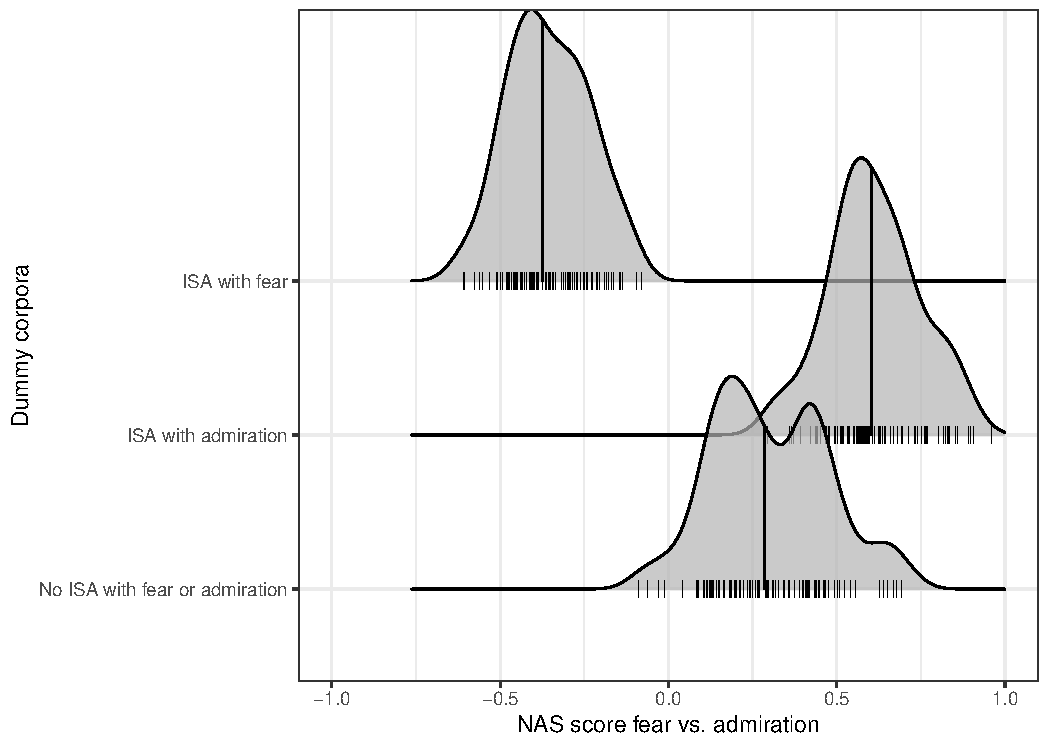
\includegraphics[width=\maxwidth]{intermediate/ridges_gg} \caption[Distribution of the NAS scores for the admiration, fear and control dummy corpora]{Distribution of the NAS scores for the admiration, fear and control dummy corpora. Negative values denote more implicit fear, positive values more implicit admiration.}\label{fig:nasplot}
\end{figure}

\end{knitrout}

The median values are diverging in the expected directions between all three dummy corpora: The admiration dummy corpus has a positive median $NAS(s, \mathcal{A}, \mathcal{B}, \boldsymbol{w})$, the fear dummy corpus a negative median, and the control dummy corpus a value between the two latter. At the same time, the control dummy corpus is closer to the admiration dummy corpus, with some overlap between the runs. This is in line with qualitative observations we made during the manual cleanup step: We found our method to generate more clearly fear-laden sentences than admiration-laden ones. Furthermore, the sentences for the control condition were not completely ``neutral'', in a sense that they did not contain any potentially emotion-eliciting words. They did, of course, not feature words from our word lists $\mathcal{A}$, $\mathcal{B}$, $\mathcal{A'}$, or $\mathcal{B'}$, yet they seemed to contain potential traces of other emotions or group-related valence. The sentences are therefore not emotionally ``neutral'' in an absolute sense, but in a relational one, meaning that they did not carry the two specific emotions fear and admiration. We deemed this sufficient for the purpose of the present validation attempt.

\subsubsection{Step 3: Measuring ISAs of the Sentence Packages as Perceived By Humans}

After testing whether our sentence packages are generating the expected ISAs within the original corpus according to word embedding-based measures, we were ready to test whether the same sentences also generate ISAs that human readers pick up. To do so, we drew a random sample of sentences for each condition---featuring 25 sentence pairs (i.e. 50 sentences in total). This additional reduction step was performed to avoid wear-out-effects and unit-non-response in participants provoked by a potentially too lengthy stimulus exposure. Our pretest showed that native German speakers read 25 sentence pairs (or 50 sentences) in less than 10 minutes. 

To still account for the semantic variance within the sentence packages, we drew three random samples of 25 sentence pairs as a stimulus package for each condition, giving us three stimulus packages of admiration sentence pairs, three stimulus packages of fear sentence pairs, and three stimulus packages of neutral sentence pairs for the control condition. In total, nine different stimulus sentence packages were created (3 ISA conditions $\times$ 3 randomized packages).\footnote{We additionally calculated $NAS$ scores for the packages of 75 sentence pairs for fear, admiration and the control condition, by merging each of them with a smaller corpus containing $\frac{1}{60^{th}}$ of all sentences of the original corpus. The resulting graph is available in Appendix F in the OSF repository.}

\textbf{Participants.} To conduct the planned 3 $\times$ 3-between-subjects experiment, we recruited a sample from the non-commercial German-language online-access panel SoSciPanel \parencite{leiner2016}. As members of this panel participate in studies without receiving incentives, they typically bring along a high intrinsic motivation to contribute to research leading to a relatively high data quality and a strong sampling bias towards high education. While this can be problematic for many types of research, we deemed it particularly advantageous for our research goal of detecting implicit associations within sentence packages as this task might require close reading. We aimed at obtaining 1,200 observations, or 133.3 observations per treatment. With this sample size, we can detect a so-called small effect size ($\eta^2$ = 0.02) at $\alpha = 0.11$ \parencite[which is the selected $\alpha$ level for the Bayesian modelling strategy, following][]{mcelreath2016} with almost 100\% statistical power. The study invitation that was sent out via e-mail to registered panel members led to an unusually high conversion rate. Thus, after data clean-up, the final sample still consisted of \textit{n} = 1937 individuals 
(48.4 \% male; 83.5 \% with highest German secondary school degree `Abitur'; age: \textit{M} = 53.3, SD = 13.9). 

\textbf{Procedure.} Upon arrival at the survey platform, participants were given detailed information about the study (without unmasking the actual research purpose) and actively consented to participation. Each participant was, then, randomly allocated to read one out of the nine stimuli. Randomization checks found no significant differences between the treatment groups regarding sociodemographics and political left-right orientation. Each stimulus contained 50 news sentences, which were displayed on five subsequent pages, presenting 10 news sentences each. All sentences were drawn in a random order from the respective stimulus sentence package during the experiment. To avoid priming effects, participants were instructed to observe the language and tonality journalists use in the sentences in general and that they would be asked to rate this language on a number of dimensions after exposure. After stimulus confrontation, the dependent variables were assessed. Finally, participants were thanked for their time and fully debriefed.

\textbf{Survey Measures.} Following stimulus exposure, we first asked participants to rate the language of the sentences they had read (e.g., concerning comprehensibility and complexity). This was included as a distraction task and to fulfill participants' expectations that they would have to rate journalists' language on multiple dimensions. Subsequently, we used one item to capture the perceived valence of the sentence packages. Similar to a feeling thermometer, we assessed the negativity/positivity participants felt the sentence package they read expressed towards the group of Italians, ranging from ``very positive'' to ``very negative'' on a 7-point scale (\textit{``How positive/negative is the portrayal of Italians in the sentences you have read?''}). This item was used to test hypotheses H1, H2 and H3. To test hypotheses H4, H5 and H6, the next two single-item measures inquired perceived admiration and perceived fear on a 7-point scale, ranging from ``very much'' to ``very little'' (\textit{``How much admiration/fear was expressed towards Italians in the sentences you have read?''}). The original German versions of all measures are available in Appendix C in the OSF repository.

\textbf{Statistical Analysis.} Following our preregistered analysis plan, we applied Bayesian Analysis of Variance to test our hypotheses \parencite{burkner2017advanced} We chose the Bayesian approach due to its pragmatic advantages yielding directly interpretable uncertainty statements about parameters, or providing only mild regularization of estimates via informative priors. We report both 1) the conditional effect and 2) the effect size $\eta^2$ and its 89\% high density intervals \parencite{easystats}. For all analyses, we used a noninformative prior of $\mathcal{N}(0,1)$. This prior assumes that before conducting our experiment there was no evidence to show $NAS(s, \mathcal{A}, \mathcal{B}, \boldsymbol{w})$ is a valid measure of ISAs conveyed to human readers in the stimulus sentence packages. Four Bayesian models for the four dependent variables perceived valence, perceived admiration, perceived fear, and assumed message effects were constructed (see Appendix D for regression coefficients and Appendix E for posterior predictive checks). For these analyses, participants exposed to either of the three different sentence packages within the same ISA condition were collapsed, leading to a total of three different analytical units. In the following, we interpret the conditional effects and the effect sizes from these models.

\section{Results}

\subsection{Perceived Valence}

\begin{knitrout}
\definecolor{shadecolor}{rgb}{0.969, 0.969, 0.969}\color{fgcolor}\begin{figure}
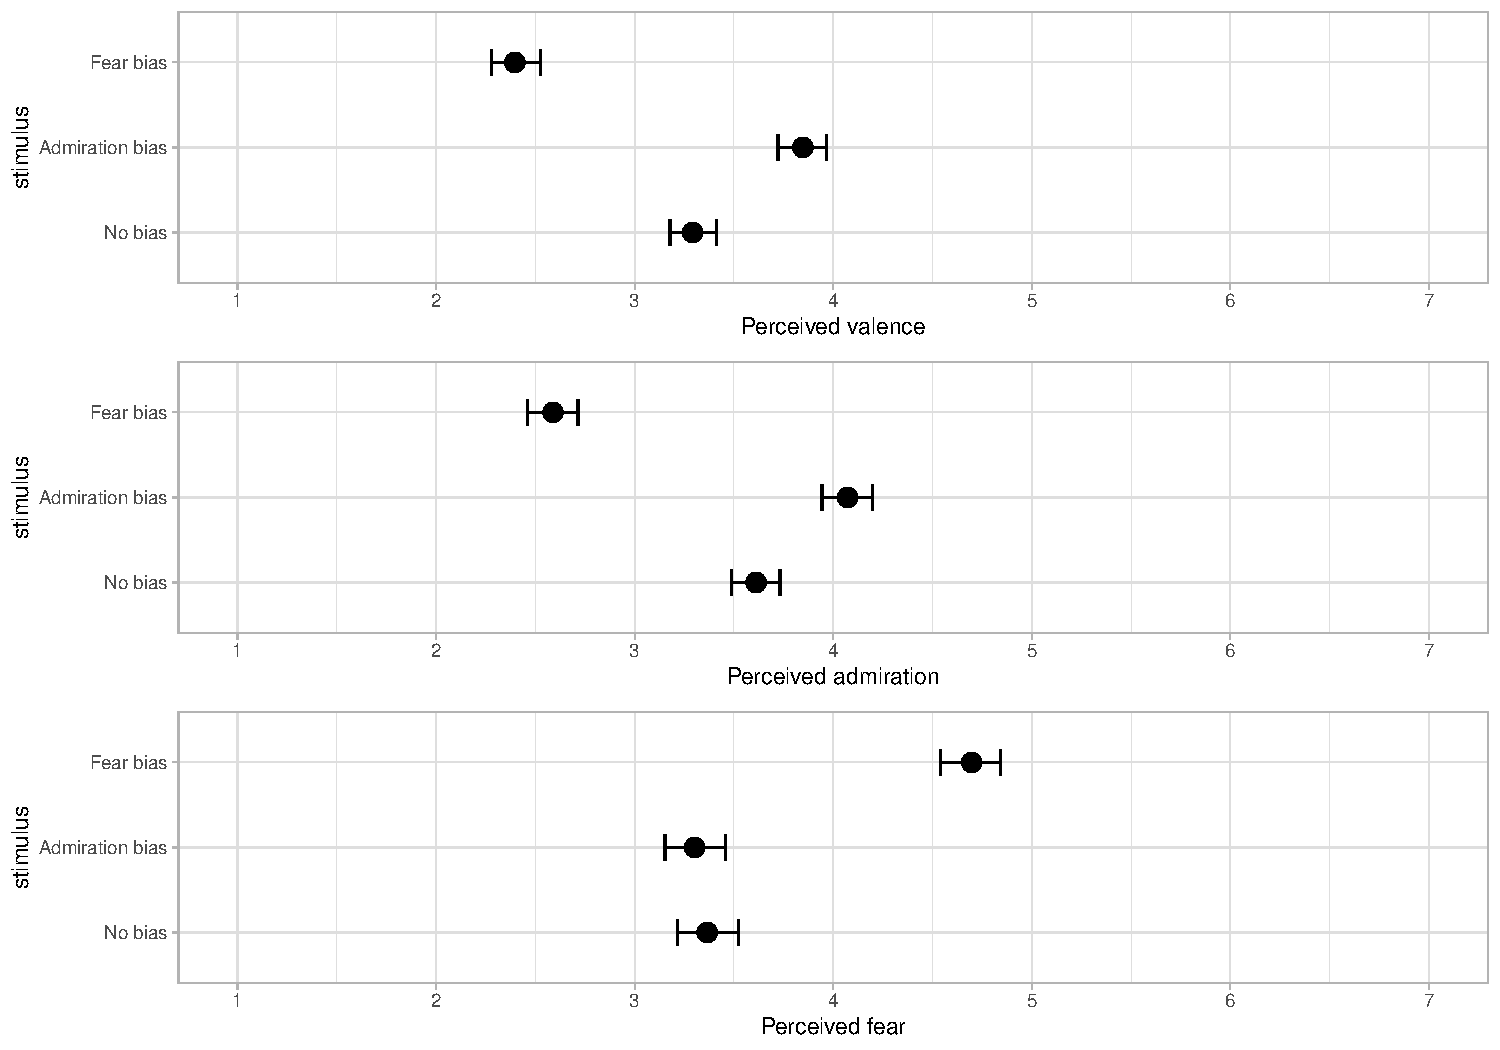
\includegraphics[width=\maxwidth]{intermediate/combined} \caption[Conditional effect plots of perceived valence (Top), perceived fear (center), and perceived admiration (bottom)]{Conditional effect plots of perceived valence (top), perceived fear (center), and perceived admiration (bottom)}\label{fig:ameplot}
\end{figure}

\end{knitrout}
Figure \ref{fig:ameplot} displays the conditional effect plots for perceived valence. The top subplot shows the conditional effect of perceived valence as a function of ISA measured for the received stimulus treatment. Results reveal that participants in the fear condition, perceived the representation of this group in the sentences they had read as much more negative than participants in the other two conditions. This supports Hs 1 and 2. Moreover, participants in the admiration condition perceived a more positive representation of the target group than those in the control condition, yielding support of H3. The effect size $\eta^2$ is 0.2 (89\% HDI: 0.17 to 0.23), and therefore much higher than the anticipated 0.02.

\subsection{Perceived Admiration}

The center subplot of Figure \ref{fig:ameplot} shows the conditional effect of perceived admiration as a function of ISA measured for the received stimulus treatment. Participants in the admiration condition perceived the representation of Italians as clearly more admirable than those in the control or fear conditions which supports H 4a and 5a. Contrary to that, participants in the fear condition found the target group presentation to convey less admiration than those in the control condition, supporting H6b. The effect size $\eta^2$ is 0.21 (89\% HDI: 0.18 to 0.25), again, much higher than the previously anticipated 0.02.

\subsection{Perceived Fear}

The bottom subplot of Figure \ref{fig:ameplot} shows the conditional effect of perceived fear as a function of ISA measured for the received stimulus treatment. Participants in the admiration condition did not perceive the representation of Italians as less frightening than individuals in the control condition. H4b is therefore not supported. However, participants in the admiration condition perceived a less frightening representation of Italians than participants in the fear condition, supporting H5b. Likewise, respondents in the fear condition perceived the representation of Italians as more frightening than those in the control condition. H6a is supported. The effect size $\eta^2$ is 0.16 (89\% HDI: 0.14 to 0.2), and, thus, once more much higher than the anticipated 0.02.

\section{Discussion}

The goal of this study was to test the semantic validity of word embedding-based measures of implicit stereotypical associations (ISAs) in large text corpora. We argued that when word embedding association measures are employed to draw conclusions about the content of these corpora---and not just as representations of exogenous cultural patterns---predictive validity does not suffice to establish that these measures allow for conclusions about the content of a study corpus. It is necessary to establish the semantic validity of these measures to be able to make claims about these texts.

To achieve this goal, we employed an experimental survey approach. This somewhat unusual validation strategy was chosen to compensate for the fact that traditional gold standard coding seemed inapplicable for the aggregated content analytical method that was to be validated in this study. Word embedding-based ISA metrics analyze implicit associations within a whole corpus in order to draw conclusions about the content of a corpus. We deemed it non-practicable for a limited number of trained human coders to make a reliable and, thus, reproducible generalizing judgment of ISAs within a whole corpus, particularly so since such associations are only implicitly present in the corpus. 

We therefore developed and employed a validation method that made use of judgments from a large number of untrained human coders assuming that, following the law of large numbers, individual participants' erroneous judgments that might possibly occur would not preponderate in this setting because the resulting patterns would regress to the (non-erroneous) mean. We conducted the data collection as a survey using typical items designed to assess given media stimuli, instead of a traditional coding task that follows a precise coding instruction. We deemed that a somewhat unreflected, more intuitive assessment of stimulus sentence packages \parencite[likely to follow a heuristic processing routine within participants;][]{chaiken1989} was actually better able to detect ISAs than the traditional coding routine for which a reflected, thorough decision-making, and, thus, systematic processing is the explicit goal. 

For demonstration purposes, we decided to use the openly available analysis corpus from a recent application of word embedding-based ISA measures for media content analysis \parencite{mueller:2023:DRN} which investigated implicit stigmatization of ethnic and religious groups in journalistic discourse, focusing on the implicit association of group labels with the emotions fear or admiration. A number of methodological decisions in this validation attempt had to be tailored to this specific study in enabling semantic validation at all. For instance, the original study \parencite{mueller:2023:DRN} covered a large variety of ethnic groups. For the purposes of our experimental semantic validation attempt, the selection of one group out of this larger variety was a crucial step to keep group-level background factors constant in the experiment. For this group, the original article corpus needed to provide a sufficient number of sentences associating it with both of the two emotions, fear and admiration. For other semantic validation attempts of word embedding-based ISA measures, other factors might be more important when choosing the right selection strategy for used sentence packages---and this will be true for multiple other methodological decisions made during the planning of the present study, depending on the design of the application that is supposed to be validated.

For instance, for studies based on one-sided word embedding bias tests \parencite{kroon2021}, finding sentences that contain the opposite valance of the measured association would be more challenging---since our approach relies on using the inverted distance to one end of the spectrum as well as the distance to the other end of the spectrum to identify clear context words. Possible solutions would be either to solely rely on the distance to the measured end of the spectrum, or to artificially construct terms that represent the implicit opposite end of the spectrum of the measured dimension. Another interesting case would be the validation of gender-stereotypes, as in \textcite{garg:2018:W}. In one of the analyses, for example, instead of measuring the association of different groups with two emotions, the authors measured the association of a large number of jobs with two genders. If a validation study of this research followed our procedure, therefore, it would have to choose a set of target occupations and construct an artificial association with different genders. This would be an interesting robustness-test for our validation procedure, as constructing artificial associations of gender with occupations can be counter-intuitive to readers who are used to opposing stereotypes---for example, it would be interesting to see if a set of stimulus sentences can suffice to induce an association counter to the observed stereotype, e.g., an association of \textit{men} with \textit{nurse}. A larger variance of target words would probably be necessary to control for more and less salient stereotypes.

Arguably, such further validation attempts are necessary. The present study constitutes just one successful validation of the application of word embedding-based ISA measures in a specific application, namely in Müller et al. (\citeyear{mueller:2023:DRN}). The between-subjects survey experiment presented in this article largely supported the assumption that participants' perception of the stimulus sentence packages was in line with the measured ISAs, thus, representing first evidence for the semantic validity of the word embedding-based approach for investigating ISAs \parencite{durrheim2023}. The successful semantic validation of an exemplary case, however, does not warrant inferences about the general semantic validity of said method. The consensus in computational communication science is that there exists no off-the-shelf method and each method requires individual validation to show the (semantic) validity for one's individual research data \parencite{atteveldt:2018:wcm,baden:2021:TGC}. Therefore, this study can only be considered a first step in establishing semantic validity of word-embedding based measures of ISAs. Further steps will necessarily have to follow, particularly when considering Krippendorff's (\citeyear[][p. 323]{krippendorff2018content}) notion that semantic validity is context dependent. Yet, if multiple other future validation studies come to similar conclusions as the present one, this could be interpreted as cumulative evidence for the general validity of word embedding-based ISA measures. But even in this case, all future applications would still require individual validation efforts.

In the specific context of the present validation, some findings call for a more in-depth engagement. For instance, the results showed that, for perceived fear as a dependent variable, there was no difference between the admiration and the no ISA stimuli. However, vice versa, perceived admiration of the target group was significantly lower in the fear stimulus condition than in the no ISA condition. This pattern does not put into question the semantic validity of the tested word embedding-based ISA measure in principle. But, it should be seen as cause to reconsider the decision to use fear and admiration as the end poles of an emotion continuum, as the preliminary work by Müller et al. (\citeyear{mueller:2023:DRN}) did. There, it was argued that the two emotions are functionally equivalent in group enhancement and devaluation in media reporting. As the present validation has shown, they are indeed causally linked, but only partially. Implicit fear-inducing messages not only increase the perceived fear of the group, but also reduce the positive emotion of admiration. Admiration-inducing messages, however, are unable to trigger a weakening of the negative emotion of fear. The communicative hurdles for overcoming fear of ethnic groups appear to be higher than those for eliminating admiration. This substantial finding of the present validation study should stimulate further research from an intergroup communication perspective. It adds a crucial facet to the discussion of the original study's results that goes beyond mere methodological validation.

Related to this, we observed another interesting pattern when constructing the sentence packages for the present validation study. A clearer difference between the control and the fear conditions could be generated, compared to the difference between the admiration and control conditions. In the survey experiment, this impression is confirmed: Participants evaluated the control sentence packages closer to the admiration packages. This observation is particularly true for the overall perceived valence of the stimuli. One explanation for this could be that the negativity bias within reporting \parencite{soroka:2015:news} leads to more cases of directly expressed fear within news reporting, while admiration is more dispersed and subtle. This could explain why the admiration sentences we found contained, at face value, less obvious traces of admiration, which both the word embedding ISA model and the participants' responses seem to confirm. This could be taken as additional evidence to challenge the decision of using fear and admiration as end poles of a two-dimensional emotion scale in Müller et al. \citeyear{mueller:2023:DRN}.

However, as the survey responses are largely in line with this pattern, they should still be interpreted as evidence for the overall semantic validity of the word embedding-based ISA measure that was tested in this study. The measure seems to be able to detect both more explicitly expressed associations (resulting in higher ISA metrics) as well as largely implicit associations (resulting in lower ISA metrics which are, yet, still distinct from zero) in line with human judgments. Thus, the present semantic validation study can be seen as supporting the general idea that word embedding based measures are able to detect ISAs in texts like human readers would. At the same time, it underscores the importance of making an informed and reflected choice about which concepts to contrast in such a necessarily bipolar measure. More broadly speaking, the observations reported here underscore the value of semantic validation, not only for ascertaining the validity of content-analytical measurements, but also for refining their conceptual underpinnings, and thus for substantial theorizing.

\subsection{Limitations and Future Research}

The present validation attempt, of course, has some limitations. First, there is the question of the scalability of its results---how representative are our constructed, relatively small sentence packages of ISA-containing sentences for naturally occurring corpora with far larger numbers of group mentions and great noise particularly within more ``neutral'' sentences? As our results indicate, we were able to construct very convincing sentence packages for the fear-association conditions---but the ``no ISA'' sentence packages, both during a face validity check and in the survey experiment, appear to contain a visible rest of ISA with emotional valence and higher semantic variance. One avenue for future research would be to find a way to scale the individual contribution of terms to the overall ISA model (both in terms of their prevalence, and in terms of their effect on the resulting ISAs) to get a more fine-grained assessment of each sentence’s actual contribution. This would allow to vary the degree of implicit association within the stimulus in a linear fashion, rather than using the current three-level ordinal ISA scale for classifying the sentence packages. 

In this study, we validated word embedding-based ISA measures for just one group that, within the original reporting, was portrayed relatively neutral with regards to the two tested emotions fear and admiration. The selection of this group was based on the assumption that implicit stereotypes towards such a group are more malleable, making it easier to measure primed perceptions of that group after exposure to a few sentence-pairs. A more complex setup would have to test whether the same semantic validation will also be successful for groups with, presumably, more established stereotypical associations with either of the two emotions fear or admiration. It may be that the experiment-based semantic validation routine presented in this study does not work for groups that are subject to strongly one-sided prejudices in public perception.

We show the concordance between $NAS(s, \mathcal{A}, \mathcal{B}, \boldsymbol{w})$ and human perceptions of ISAs within a sentence package among the three specified levels (admiration, fear, and no ISA) through which we provide evidence of semantic validity. However, this approach does not provide any evidence on the calibration \parencite{lindhiem:2018:ICC} of $NAS(s, \mathcal{A}, \mathcal{B}, \boldsymbol{w})$, i.e. how the difference between any two arbitrary points on the scale of $NAS(s, \mathcal{A}, \mathcal{B}, \boldsymbol{w})$ actually corresponds to the human perception of difference in the fear-admiration dichotomy. One possible solution to show the calibration of word embedding-based ISA measures is the rich stimulus sampling approach proposed by \textcite{young:2011:R}. Under that approach, a stimulus (dummy corpus and its stimulus sentence packages) should be randomly generated on the fly and therefore the level of ISA would not be preconfigurated.

Another limitation could be seen in the participant sample used for the present study. Perceptions of the stereotype intensity conveyed by the same implicit associations plausibly vary with political orientation, lived experience (including being a target of stereotyping), socio-economic and cultural–linguistic background. For example, Italian immigrants may read the affective implications differently than members of the ethnic majority in Germany. This raises a normative question: Whose perceptions should count in semantic validation? The present experiment establishes semantic validity for a reference population that is somewhat skewed towards higher education, but diverse in terms of other socio-demographic factors and political attitudes \parencite{leiner2016}. Considering that typical gold-standard validation studies often rely exclusively on highly educated student assistants who are even less diverse in terms of political orientation and age than our sample, we deemed the dominance of highly educated individuals in the sample acceptable. However, one could argue that, if the goal is to assess the reception of a general audience, a truly representative sample is required as a next step. If the goal is to assess potential harm, it would be advisable to oversample targeted groups. Semantic validation studies employing an experimental approach should therefore carefully consider which kind of benchmark they are aiming for and what participant sample structure is required to achieve it.

Finally, it has to be mentioned that the approach to measuring ISAs which we semantically validated in the present study uses so-called static word embeddings such as GLoVE. However, there are also newer models (e.g., BERT, ELMO, and GPT) which allow to generate so called contextual word embeddings. Methods such as WEAT have been extended by the original authors recently to cover contextual word embeddings \parencite{guo:2021:DEI} and there appear to be new applications of contextual word embeddings in communication research \parencite{thijs:2024:CWE}. The evidence of semantic validity presented in this article is certainly not directly transferable to ISAs measured using contextual word embeddings. Yet, its survey experimental approach can be used as the basis to validate ISAs found through contextual word embeddings, too. For this purpose, one might need to take the multi-level approach by \textcite{guo:2021:DEI} to 1) generate the same set of stimuli for various contexts, and then 2) combine the effect sizes from different contexts using a random-effect model.

At the same time, newer word embedding methods could ease validation in terms of the required computational effort: When conducting the present analysis based on GLoVE word embeddings, our main analysis took seven days to compute, while the robustness-check took about five weeks on a university HPC to run. This process could be sped up significantly with word-embedding models that are optimized for running on graphics cards instead of CPUs, allowing for a larger variance of parameters and combinations of contexts to be included in the analysis at sensible timescales for analysis.

\section{Conclusion}

Despite the aforementioned limitations, the present results are more than encouraging for the application of a word embedding-based corpus-level metrics in the domain of computational communication analysis. While previous research had already tested the statistical and predictive validity of word embedding-based ISA detection methods \parencite{durrheim2023}, we complemented the picture with the present study, offering first evidence for their semantic validity. This should be read as further consolidation for the assumption that word embedding models are able to capture and quantify actual implicit associations within text corpora as perceived by human readers. For the time being, a broader application of this method for the measurement of various kinds of associations within media (and other) texts does seem promising. However, researchers applying word embedding-based metrics in the future should, of course, be aware that the present semantic validation (even in conjunction with previous statistical and predictive validations of the method) may be limited in its transferability to other research domains.

\section{Acknowledgments}

This research was supported by the German Federal Ministry for Family Affairs, Senior Citizens, Women and Youth (BMFSFJ) through a grant to the ``Research Association Discrimination and Racism'' (FoDiRa) of the DeZIM-Research Community (German Center for Integration and Migration Research).

%\printbibliography
